\section{代数连通度}
\label{sec:graph-algebraic-connectivity}

判断一张图是否连通，只需要检查任意两个顶点之间是否存在路径；但要刻画一张连通图“连得有多稳固”，则需要审视它的全局几何形态。本节先通过四类典型图建立“瓶颈”与“稀疏割”的几何图像，再对比局部组合连通度与全局稀疏割度量的局限，由此引出连续可算的代数连通度$\lambda_2$及其对应的Fiedler向量$\bm v_2$。

\subsection{连通度的几何意义}
\label{sec:graph-connectivity-geometry}

连通性只判断任意两点之间是否存在路径。对于已经连通的图，还可以考察删除多少条边会使它断开，以及断开后两侧的规模。图~\ref{fig:graph-connectivity-archetypes}通过四类图比较这些性质。

\begin{BookInlineFigure}
  \centering
  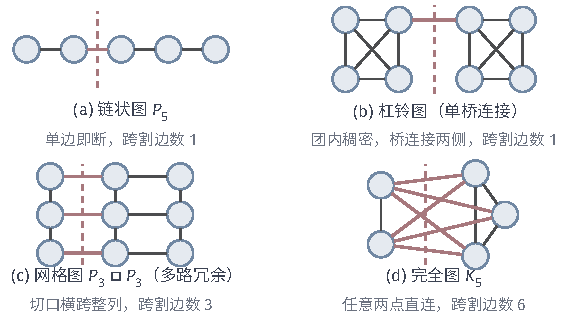
\includegraphics[width=96.238mm]{figures/03-graphs/05-matrices-and-spectra/tikz/connectivity-four-archetypes/figure.pdf}
  \caption{四类典型连通图的瓶颈结构对比。红色虚线标出将图切分为两个较大子集的最薄弱切口，红色实线为被切断的跨割边。(a) 链状图任一内边都是唯一通路；(b) 杠铃图两侧稠密但受制于中间的细腰单桥；(c) 网格图有多条平行通路，切口需横跨整列；(d) 完全图任意两部分之间都有密集边相连。}
  \label{fig:graph-connectivity-archetypes}
\end{BookInlineFigure}

第一类是\emph{链状图}（路径图$P_n$，$n\geq2$）。任意两点之间只有一条路径；删除任意一条边，或在$n\geq3$时删除任意内部顶点，都会使图分为两个连通分量。

第二类是\emph{杠铃图}（barbell graph）。这里取两个完全子图通过一条桥边相连的形式。两个子图内部均有较多连接，但删除中间的桥边就会使两侧断开。因此，局部边数较多并不保证全图没有规模较大的稀疏割。

第三类是\emph{网格图}$P_m\square P_m$（$m\geq2$）。它有$n=m^2$个顶点，每个内部顶点有四个邻居。沿相邻两列之间切开需要删除$m$条边；当$m$为偶数且从中间切开时，两侧顶点数相等。这个例子说明，某些图的均衡切分需要切断随规模增长的多条边。

第四类是\emph{完全图}$K_n$。将顶点集分成大小为$s$和$n-s$的两部分时，割边数为$s(n-s)$。当两侧大小都与$n$同阶时，割边数为$\Theta(n^2)$；若只隔离一个顶点，则只需删除$n-1$条边。讨论切分代价时，需要同时说明两侧的规模。

这些例子提示我们用\emph{稀疏割}（sparse cut）描述图中的连接瓶颈。对非空真子集$S\subsetneq V$，跨割边权为$c(S,\bar S)=\sum_{i\in S,j\in\bar S}w_{i,j}$。只有将它与两侧规模比较，才能区分“隔离一个低度顶点”和“分开两个较大的子图”。后面分别用顶点数与度数总和衡量规模，得到不同的稀疏割指标。

\subsection{连通度的度量}
\label{sec:graph-connectivity-measures}

如何将上述“瓶颈/稀疏割”的几何直觉转化为精确的数学度量？传统图论与组合优化分别从“最弱局部脱节代价”和“全局归一化割代价”两个角度提出了不同的指标，但二者在刻画能力与计算复杂度上各自面临根本困难。

\paragraph{局部组合连通度：$\kappa(\mathcal G)$、$\lambda(\mathcal G)$与$\delta(\mathcal G)$}

在经典图论中，简单无权图$\mathcal G=(V,E)$的连通程度通常由三个离散组合量来度量。第一个量是\term{点连通度}（vertex connectivity）$\kappa(\mathcal G)$，定义为使图变得不连通（或缩为单个顶点）所需删去的最少顶点数。第二个量是\term{边连通度}（edge connectivity）$\lambda(\mathcal G)$，定义为使图变得不连通所需删去的最少边数，即所有非空真子集割的最小割边数：
\begin{equation}
\label{eq:graph-edge-connectivity-def}
  \lambda(\mathcal G) = \min_{\varnothing\neq S\subsetneq V} c(S,\bar S).
\end{equation}
（注意此处带括号的$\lambda(\mathcal G)$表示图$\mathcal G$的边连通度，勿与带下标的拉普拉斯特征值$\lambda_1\leq\lambda_2\leq\cdots\leq\lambda_n$混淆。）第三个量是全图的\term{最小度数}（minimum degree）$\delta(\mathcal G)=\min_{v\in V}d_v$。

对任意顶点$v\in V$，只要删去与$v$关联的全部$d_v$条边，就能将单点$\{v\}$与其余顶点彻底隔开，因此必有$\lambda(\mathcal G)\leq\delta(\mathcal G)$；进一步，从最小边割的每条跨边中适当选取端点删去，又可证明$\kappa(\mathcal G)\leq\lambda(\mathcal G)$（详见定理~\ref{thm:graph-connectivity-comparison}）。三者满足经典的Whitney不等式：
\begin{equation}
\label{eq:graph-whitney-inequality}
  \kappa(\mathcal G) \leq \lambda(\mathcal G) \leq \delta(\mathcal G).
\end{equation}

点连通度$\kappa(\mathcal G)$与边连通度$\lambda(\mathcal G)$都是对全图取最小得到的量，但不记录最小分隔造成的两侧规模。图~\ref{fig:graph-connectivity-local-vs-global}中，$K_5$外接一个叶子与两个$K_4$经单桥相连的图均满足$\kappa=\lambda=1$；前者的最小边割隔离一个顶点，后者则把图分成等大的两部分。这两个指标本身不能区分这两种切分。

\begin{BookInlineFigure}
  \centering
  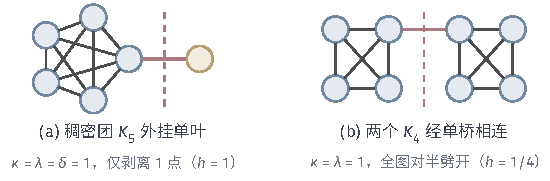
\includegraphics[width=93.059mm]{figures/03-graphs/05-matrices-and-spectra/tikz/connectivity-local-vs-global/figure.pdf}
  \caption{点、边连通度$\kappa(\mathcal G),\lambda(\mathcal G)$与等周数$h(\mathcal G)$的对比。(a) 稠密团$K_5$外挂单个叶子顶点，最弱局部切口仅剥离$1$个末梢顶点；(b) 两个$K_4$经单条桥边相连，最弱切口将全图对半劈开。两张图的$\kappa(\mathcal G)=\lambda(\mathcal G)=1$完全相同，但全局等周数分别为$h=1$与$h=1/4$。}
  \label{fig:graph-connectivity-local-vs-global}
\end{BookInlineFigure}

上述无权连通度只依赖边是否存在，不反映已有边的权重变化。若要比较加权网络，还需要采用割权或谱量。加权最小割值是若干线性函数的最小值，随边权连续变化，但在最优割改变时可能不可微；代数连通度也可能在特征值重合处不可微，因此连续性与可微性应分别讨论。

\paragraph{全局稀疏割指标与NP-Hard计算困境}

为了真正捕捉全局瓶颈，必须在跨割边代价$c(S,\bar S)$的分母上除以两侧子集的规模，迫使指标同时兼顾“割边少”与“两侧大”。按顶点数衡量集合规模时，最自然的全局稀疏割指标是图的\term{等周数}（isoperimetric number，亦称\term{Cheeger常数}）：
\begin{equation}
\label{eq:graph-isoperimetric-number}
  h(\mathcal G) = \min_{\varnothing\neq S\subsetneq V} \frac{c(S,\bar S)}{\min\{|S|,|\bar S|\}},
\end{equation}
以及对称兼顾两侧顶点数的\term{比例割}（RatioCut）：
\begin{equation}
\label{eq:graph-ratiocut-preview}
  \operatorname{RatioCut}(S) = c(S,\bar S)\left(\frac{1}{|S|}+\frac{1}{|\bar S|}\right).
\end{equation}
若改按度数总和（集合体积$\operatorname{vol}(S)=\sum_{i\in S}d_i$）衡量规模，则得到第~\ref{sec:graph-cheeger}节将深入研究的导通率$\phi(S)$与第~\ref{sec:graph-ncut}节的归一化割$\operatorname{NCut}(S)$。

在图~\ref{fig:graph-connectivity-local-vs-global}中，图(a)切下单叶时$\min\{|S|,|\bar S|\}=1$，等周数$h(\mathcal G)=1/1=1$；而图(b)沿桥边对半切开时$\min\{|S|,|\bar S|\}=4$，等周数为$h(\mathcal G)=1/4$，反映了两侧规模不同所带来的指标差异。

然而，这种全局精准性付出了高昂的计算代价：在包含$n$个顶点的图上，非空无序二分共有$2^{n-1}-1$种；精确求解最小等周数$h(\mathcal G)$、最小导通率$\phi_*$或最小RatioCut，均已被证明是\emph{NP-Hard组合优化难题}。当图的顶点数达到数千乃至数百万时，遍历所有离散子集寻找最稀疏割在计算上完全不可行。

因此可以考虑连续松弛：用能够高效近似计算的特征值给出离散割目标的界，再从特征向量构造候选划分。

\subsection{代数连通度}
\label{sec:graph-algebraic-connectivity-variational}

这个连续可算替代品正是组合拉普拉斯矩阵$\bm L=\bm D-\bm W$的第二小特征值$\lambda_2$。为了理解$\lambda_2$为何能度量全局连通程度，我们先从拉普拉斯二次型的沿边能量出发给出它的定义与变分刻画，再证明它与经典连通度及全局稀疏割的定量关系。

\paragraph{代数连通度的定义与变分刻画}

回顾第~\ref{sec:graph-laplacian-energy}节，给每个顶点$i$赋予实数值$x_i$时，组合拉普拉斯二次型
\[
  \bm x^\top\bm L\bm x = \sum_{\{i,j\}\in E} w_{i,j}(x_i-x_j)^2
\]
累加了所有边两端读数差的平方，衡量向量$\bm x$在图上的沿边变化能量。例如在图~\ref{fig:graph-partition-edge-energy}(a)的单位权四点路径上，给前两个顶点赋$+1$、后两个赋$-1$，只有中间边$23$产生差值$1-(-1)=2$，总能量为$4$；而在图~\ref{fig:graph-partition-edge-energy}(b)中添入跨接首尾的边$14$后，同一赋值的总能量增至$8$。

\begin{BookInlineFigure}
  \centering
  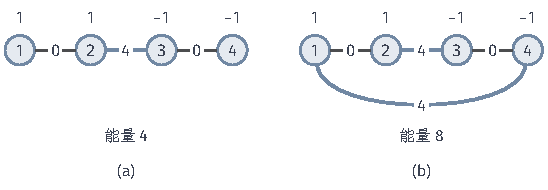
\includegraphics{figures/03-graphs/05-matrices-and-spectra/tikz/partition-edge-energy/figure.pdf}
  \caption{对同一组顶点赋值计算沿边能量。(a) 四点路径，只有中间边贡献了能量$4$。(b) 加上边$14$后得到四边环，新增的边上也有差$2$，总能量变为$8$。顶点上方是赋值，边上的数是差的平方。}
  \label{fig:graph-partition-edge-energy}
\end{BookInlineFigure}

要在给定图上寻找“沿边能量最小”的非平凡顶点赋值，必须满足两条规范化约束。第一，给所有顶点赋相同的常数时，每条边两端差均为零，能量恒为零；这种常值赋值不反映任何图结构信息，因此需要要求赋值向量与全一常向量正交，即满足零和条件$\bm x\perp\bm 1$（$\sum_{i=1}^n x_i=0$）。

第二，将非零向量$\bm x$同乘常数$c\neq 0$会使能量$\bm x^\top\bm L\bm x$与欧氏长度平方$\bm x^\top\bm x$同步放大$c^2$倍；为了在同一尺度下公平比较不同方向，应当考察两者的比值——即Rayleigh商$\frac{\bm x^\top\bm L\bm x}{\bm x^\top\bm x}$。Fiedler于1973年提出将非平凡方向上的最小Rayleigh商定义为图的代数连通度。

\begin{definition}[代数连通度]
\label{def:graph-algebraic-connectivity}
设$n$阶无向非负加权图$\mathcal G$的组合拉普拉斯矩阵$\bm L$的特征值按升序排列为$0=\lambda_1\leq\lambda_2\leq\cdots\leq\lambda_n$。图的\term{代数连通度}（algebraic connectivity）定义为第二小特征值$\lambda_2(\mathcal G)$（在不致混淆时简记为$\lambda_2$），其Courant--Fischer变分刻画为
\begin{equation}
\label{eq:graph-algebraic-connectivity}
\lambda_2
=\min_{\substack{\bm x\perp\bm 1\\\bm x\ne\bm 0}}
\frac{\bm x^\top\bm L\bm x}{\bm x^\top\bm x}
=\min_{\substack{\bm x^\top\bm 1=0\\\lVert\bm x\rVert_2=1}}
\bm x^\top\bm L\bm x.
\end{equation}
\end{definition}

将式~\eqref{eq:graph-algebraic-connectivity}与前文的正交特征展开相对照，可以一步看清该极小值的代数结构。设$\bm v_1=\bm 1/\sqrt{n},\bm v_2,\ldots,\bm v_n$为$\bm L$对应于$0=\lambda_1\leq\lambda_2\leq\cdots\leq\lambda_n$的标准正交特征向量基。

任取满足$\bm x\perp\bm 1$的非零向量$\bm x$，它在$\bm v_1$方向上的投影系数为零，故可展开为$\bm x=\sum_{k=2}^n\alpha_k\bm v_k$。

代入Rayleigh商并利用特征向量的正交性，可得
\[
  \frac{\bm x^\top\bm L\bm x}{\bm x^\top\bm x}
  = \frac{\sum_{k=2}^n\lambda_k\alpha_k^2}{\sum_{k=2}^n\alpha_k^2}
  \geq \lambda_2,
\]
且当$\bm x$取为$\lambda_2$对应的特征向量$\bm v_2$时等号精确成立。

由这一变分刻画立即可读出代数连通度的三项基本性质：
\begin{enumerate}
\item \emph{连通性的充要判据}：由第~\ref{sec:graph-laplacian-kernel}小节知，$\bm L$的零特征值重数等于图$\mathcal G$的连通分量个数。因此$\lambda_2>0$当且仅当$\mathcal G$连通；$\lambda_2=0$当且仅当$\mathcal G$不连通。
\item \emph{关于边权与加边的单调性}：若在相同顶点集上增大边权或添加新边得到$\mathcal G'$，则对每个零和向量$\bm x$都有$\bm x^\top\bm L(\mathcal G')\bm x\geq\bm x^\top\bm L(\mathcal G)\bm x$，取最小后即得$\lambda_2(\mathcal G')\geq\lambda_2(\mathcal G)$。
\item \emph{典型图族的定量对比}：结合第~\ref{sec:graph-typical-laplacian-spectra}小节算出的典型图谱，四类典型图（图~\ref{fig:graph-connectivity-archetypes}）的代数连通度呈现出鲜明的量级差异：链状路径图$\lambda_2(P_n)=2\bigl(1-\cos(\pi/n)\bigr)=\Theta(n^{-2})$，随$n$增大迅速衰减至$0$；由两个$K_m$经单桥相连的杠铃图（$m\geq2$，$n=2m$）满足$\lambda_2=\bigl(m+2-\sqrt{(m+2)^2-8}\bigr)/2=\Theta(m^{-1})=\Theta(n^{-1})$，定量暴露出细腰瓶颈；二维网格图$\lambda_2(P_m\square P_m)=2\bigl(1-\cos(\pi/m)\bigr)=\Theta(n^{-1})$，比链状图高出一个量级；而完全图$\lambda_2(K_n)=n$随规模线性增长，成为所有$n$阶简单无权图的上界。
\end{enumerate}

\paragraph{代数连通度与其他连通度的关系}

代数连通度$\lambda_2$不仅在定性趋势上区分了不同图族，而且与前文介绍的局部组合连通度$\kappa(\mathcal G),\lambda(\mathcal G),\delta(\mathcal G)$以及全局稀疏割指标$h(\mathcal G),\operatorname{RatioCut}$之间存在严格的不等式联系。我们先证明Fiedler关于局部连通度的经典上界定理。

\begin{theorem}[代数连通度与点、边连通度的比较]
\label{thm:graph-connectivity-comparison}
设$\mathcal G=(V,E)$为有限简单无权连通非完全图，则其代数连通度$\lambda_2(\mathcal G)$、点连通度$\kappa(\mathcal G)$、边连通度$\lambda(\mathcal G)$与最小度数$\delta(\mathcal G)$满足
\begin{equation}
\label{eq:graph-connectivity-comparison}
  \lambda_2(\mathcal G)\leq\kappa(\mathcal G)\leq\lambda(\mathcal G)\leq\delta(\mathcal G).
\end{equation}
\end{theorem}

\begin{proof}
我们按从左到右的顺序分三步证明式~\eqref{eq:graph-connectivity-comparison}中的三个不等号。

第一步：证明$\lambda_2(\mathcal G)\leq\kappa(\mathcal G)$。因为$\mathcal G$是连通非完全图，必存在最小点分隔集$T\subsetneq V$（$|T|=\kappa(\mathcal G)$），使得删去$T$后剩余顶点集$V\setminus T$至少分裂为两个互不相连的非空部分。取其中一个连通块记为$A$，将其余所有块合并记为$B=V\setminus(T\cup A)$，则$A,B$均非空，且$A$与$B$之间没有任何直接边相连。

构造如下三值试探向量$\bm x\in\mathbb R^n$：对$i\in A$令$x_i=|B|$，对$i\in B$令$x_i=-|A|$，对$i\in T$令$x_i=0$。

核对零和条件：$\bm x$的各分量之和为
\[
  \sum_{i=1}^n x_i = |A|\cdot|B| + |B|\cdot(-|A|) + |T|\cdot 0 = 0,
\]
故$\bm x\perp\bm 1$且$\bm x\neq\bm 0$。

计算分母的欧氏长度平方：
\[
  \bm x^\top\bm x = |A|\cdot|B|^2 + |B|\cdot|A|^2 = |A||B|(|A|+|B|).
\]

计算分子的沿边能量$\bm x^\top\bm L\bm x$：$A$内部各点取值恒为$|B|$，差为零；$B$内部各点取值恒为$-|A|$，差为零；$T$内部各点取值恒为$0$，差也为零；而$A$与$B$之间无边。因此，只有一端在$T$、另一端在$A$或$B$的边才对能量有贡献。

由于$\mathcal G$是简单无权图，$A$中的每个顶点至多与$T$中的$|T|$个顶点相邻，每条这样的边贡献$(|B|-0)^2=|B|^2$；同理，$B$中的每个顶点至多与$T$中的$|T|$个顶点相邻，每条这样的边贡献$(-|A|-0)^2=|A|^2$。累加可得分子上界：
\[
  \bm x^\top\bm L\bm x
  \leq |T|\bigl(|A|\cdot|B|^2 + |B|\cdot|A|^2\bigr)
  = |T|\cdot|A||B|(|A|+|B|).
\]

将分子上界除以分母$\bm x^\top\bm x$，结合变分刻画式~\eqref{eq:graph-algebraic-connectivity}即得
\[
  \lambda_2(\mathcal G)\leq\frac{\bm x^\top\bm L\bm x}{\bm x^\top\bm x}\leq |T|=\kappa(\mathcal G).
\]

第二步：证明$\kappa(\mathcal G)\leq\lambda(\mathcal G)$。取一个大小为$\lambda(\mathcal G)$的最小边割$c(S,\bar S)$。若在两侧能找到一对不相邻的顶点$u\in S$与$v\in\bar S$，则每条跨割边至少有一个端点不属于$\{u,v\}$；从每条跨割边各选一个异于$u,v$的端点组成集合$T$，则$|T|\leq\lambda(\mathcal G)$且删去$T$即切断了$u$与$v$之间的所有跨边，故$\kappa(\mathcal G)\leq|T|\leq\lambda(\mathcal G)$。

若$S$与$\bar S$之间的所有可能边都存在，设$|S|=p,|\bar S|=q$，则$\lambda(\mathcal G)=pq$；由$(p-1)(q-1)\geq 0$知$pq\geq p+q-1=n-1$，而在非完全图中任取一对不相邻顶点并删去其余$n-2$个顶点即可断开图，故仍有$\kappa(\mathcal G)\leq n-2<n-1\leq\lambda(\mathcal G)$。

第三步：证明$\lambda(\mathcal G)\leq\delta(\mathcal G)$。取达到最小度数的顶点$v_0$（$d_{v_0}=\delta(\mathcal G)$），令$S=\{v_0\}$，则割$(S,\bar S)$恰好切断与$v_0$关联的$\delta(\mathcal G)$条边，故$\lambda(\mathcal G)\leq c(\{v_0\},V\setminus\{v_0\})=\delta(\mathcal G)$。
\end{proof}

在单位权四点路径$P_4$上，$\lambda_2=2-\sqrt 2\approx 0.586<\kappa(P_4)=\lambda(P_4)=\delta(P_4)=1$；在四元环$C_4$上，$\lambda_2=\kappa(C_4)=\lambda(C_4)=\delta(C_4)=2$，不等式链全部取等（图~\ref{fig:graph-connectivity-separator-trial}）。完全图$K_n$之所以在定理~\ref{thm:graph-connectivity-comparison}中单独排除，是因为$K_n$中不存在不相邻的顶点对，无法删点将其分成两个不相连的非空部分，按约定$\kappa(K_n)=\lambda(K_n)=\delta(K_n)=n-1$，而$\lambda_2(K_n)=n$。

\begin{BookInlineFigure}
  \centering
  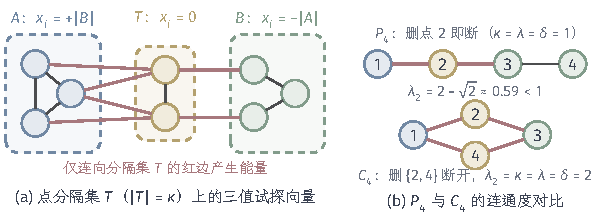
\includegraphics[width=102.164mm]{figures/03-graphs/05-matrices-and-spectra/tikz/connectivity-separator-trial/figure.pdf}
  \caption{点分隔集试探向量构造与连通度不等式核对。(a) 删去最小点分隔集$T$（$|T|=\kappa$）将图分为互不相连的$A$与$B$；给$A$赋$+|B|$、$B$赋$-|A|$、$T$赋$0$后，仅连向$T$的红边产生沿边能量。(b) $P_4$（严格不等式）与$C_4$（等号成立）的连通度对比。}
  \label{fig:graph-connectivity-separator-trial}
\end{BookInlineFigure}

除了受局部连通度$\kappa(\mathcal G)$上界控制之外，代数连通度$\lambda_2$还直接给出了全局等周数$h(\mathcal G)$与最小RatioCut的\emph{连续下界}。对任意非空真子集$S\subsetneq V$（记$s=|S|,t=|\bar S|=n-s$），在式~\eqref{eq:graph-algebraic-connectivity}中代入中心化两值试探向量$\bm y=\bm 1_S-\frac{s}{n}\bm 1$（详见第~\ref{sec:graph-ratiocut-relaxation}小节定理~\ref{prop:graph-ratiocut-relaxation}），立即可得
\begin{equation}
\label{eq:algebraic-connectivity-isoperimetric-bound}
  \lambda_2(\mathcal G)
  \leq \frac{\bm y^\top\bm L\bm y}{\bm y^\top\bm y}
  = c(S,\bar S)\left(\frac{1}{|S|}+\frac{1}{|\bar S|}\right)
  = \operatorname{RatioCut}(S)
  \leq \frac{2\,c(S,\bar S)}{\min\{|S|,|\bar S|\}}.
\end{equation}
对所有非空真子集$S$取最小后，即得全局稀疏割的下界关系：
\begin{equation}
\label{eq:algebraic-connectivity-cheeger-lower}
  \frac{\lambda_2(\mathcal G)}{2}
  \leq \frac{1}{2}\min_{\varnothing\neq S\subsetneq V}\operatorname{RatioCut}(S)
  \leq h(\mathcal G).
\end{equation}
式~\eqref{eq:algebraic-connectivity-cheeger-lower}给出了按顶点数归一化的割权下界：$h(\mathcal G)\geq\lambda_2/2$。这里的尺度仍依赖边权；把全部边权同乘常数会使$\lambda_2$和$h$同比变化。若希望指标对这种整体缩放不变，可以改用度加权体积作分母，这将引出下一节的导通率与归一化拉普拉斯。

\subsection{Fiedler向量}
\label{sec:graph-fiedler-vector}

代数连通度$\lambda_2$给出割权的谱下界，而相应的特征向量$\bm v_2$提供一维顶点坐标，可据此构造候选划分。它一般不直接给出最优稀疏割。

\begin{definition}[Fiedler向量]
\label{def:graph-fiedler-vector}
设连通无向非负加权图$\mathcal G$的组合拉普拉斯矩阵为$\bm L$。对应于代数连通度$\lambda_2>0$的非零特征向量$\bm v_2$（即满足$\bm L\bm v_2=\lambda_2\bm v_2$且$\bm v_2^\top\bm 1=0$，亦常记作$\bm f$）称为图的\term{Fiedler向量}（Fiedler vector）。
\end{definition}

如果$\lambda_2$是单重特征值，单位长度的Fiedler向量在差一个正负号的意义下唯一确定；若$\lambda_2$为重根，则对应的特征子空间中任意非零向量都是Fiedler向量。由于连通图上$\bm v_2\perp\bm 1$，Fiedler向量的所有分量之和为零：$\sum_{i=1}^n(\bm v_2)_i=0$，因此它必然同时包含正分量与负分量。

\paragraph{Fiedler向量$\bm v_2$的物理与几何意义}

我们可以从弹簧势能、振动和扩散三个角度理解$\bm v_2$为何可用于构造划分。

第一个视角是\emph{一维胡克弹簧网络的最小势能嵌入}。将图中的每条边$\{i,j\}$看作劲度系数为$w_{i,j}$的理想弹簧，把每个顶点$i$放置在实数轴上的坐标$x_i=(\bm v_2)_i$处，则拉普拉斯二次型的一半$\frac12\bm x^\top\bm L\bm x=\frac12\sum_{\{i,j\}\in E}w_{i,j}(x_i-x_j)^2$恰好是整个弹簧系统的总弹性势能。零和条件$\sum_i x_i=0$将全部顶点的重心固定在原点$0$，单位长度条件$\sum_i x_i^2=1$则固定了顶点在实轴上的总展开尺度，防止所有顶点坍缩到原点以逃避势能。

在零和与单位长度约束下，最小化Rayleigh商等价于最小化上述弹簧势能。图~\ref{fig:graph-fiedler-barbell}中的两个三角形仅由边$3\!-\!4$连接，其Fiedler向量在两个三角形上分别取负值和正值，团内坐标差小于桥边两端的坐标差。这说明该图的低能量方向能够反映桥边所连接的两个部分；对于一般图，仍须计算各候选割的目标值来判断划分质量。

\begin{BookInlineFigure}
  \centering
  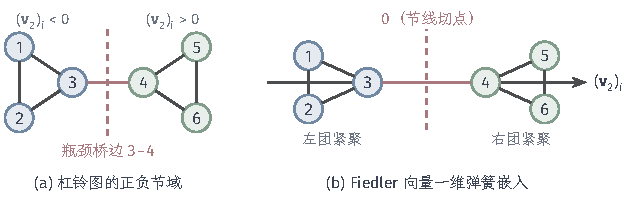
\includegraphics[width=107.495mm]{figures/03-graphs/05-matrices-and-spectra/tikz/fiedler-barbell-embedding/figure.pdf}
  \caption{杠铃图上Fiedler向量$\bm v_2$的物理意义与一维弹簧嵌入。(a) 两个三角形团$\{1,2,3\}$与$\{4,5,6\}$经单条瓶颈桥边$3\!-\!4$相连，$\bm v_2$在左团取负值、右团取正值；(b) 将顶点放置在实轴坐标$(\bm v_2)_i$上时，团内密集弹簧将各自顶点紧紧聚拢在两侧，唯一的瓶颈桥边被大幅拉伸并跨越原点$0$（红色虚线切点）。}
  \label{fig:graph-fiedler-barbell}
\end{BookInlineFigure}

第二个视角是\emph{弹性振动的基频驻波模态}。在质量均匀的离散振动网络$\frac{\mathrm d^2\bm u}{\mathrm dt^2}=-\bm L\bm u$中，$\lambda_1=0$对应全体顶点同向平移的刚体运动（零频模态），而$\lambda_2>0$对应的$\bm v_2$则是系统的第一阶非平凡简谐振动模态（基频驻波）。正负分量表示相反的振动相位，角频率为$\sqrt{\lambda_2}$。在上述杠铃图中，两团以相反相位振动；一般图的符号边界不保证对应最优稀疏割。

第三个视角是\emph{图上热扩散的最慢衰减模态}。在连续时间热传导或共识扩散方程$\frac{\mathrm d\bm x}{\mathrm dt}=-\bm L\bm x$中，任意初始温度分布$\bm x(0)=\sum_{k=1}^n\alpha_k\bm v_k$按$\bm x(t)=\alpha_1\bm v_1+\sum_{k=2}^n\alpha_k\mathrm e^{-\lambda_k t}\bm v_k$演化。非恒定模态按各自的$\mathrm e^{-\lambda_k t}$衰减，最小正特征值$\lambda_2$对应最慢衰减率。若$\lambda_2$为重特征值，整个对应特征子空间具有相同的衰减率；该部分是否出现在演化中，还取决于初值在此子空间上的投影。

\paragraph{Fiedler节域连通性定理}

按Fiedler向量的符号可以构造二分候选。下面的Fiedler节域连通性定理保证非负顶点集和非正顶点集各自诱导连通子图；这是一项连通性结论，不是割目标最优性的保证。

\begin{theorem}[Fiedler节域连通性定理]
\label{thm:graph-fiedler-connected-side}
设有限无向加权图$\mathcal G$的正权支撑连通，$\bm f=\bm v_2$为组合拉普拉斯矩阵$\bm L$的Fiedler向量。则非负顶点集合$V_+=\{i\in V:f_i\geq 0\}$（以及对称地，非正顶点集合$V_-=\{i\in V:f_i\leq 0\}$）所诱导的正权子图必定连通。
\end{theorem}

\begin{proof}
由$\bm f$与$-\bm f$的对称性，只需证明$V_+=\{i:f_i\geq 0\}$诱导的正权子图连通。反设$V_+$分裂成了两个或更多个互不连通的连通块，我们将导出矛盾。

第一步：写出单个非负连通块上的特征方程。记严格负值顶点集合为$N=\{j\in V:f_j<0\}$，任取$V_+$的一个连通块$C$。由于$V_+$的不同连通块之间没有正权边相连，特征方程$\bm L\bm f=\lambda_2\bm f$限制在块$C$的坐标上只涉及$C$自身与负值集$N$：
\[
  \bm L_{C,C}\bm f_C = \lambda_2\bm f_C - \bm r_C,
  \qquad
  \bm r_C = \bm L_{C,N}\bm f_N.
\]
矩阵块$\bm L_{C,N}$的元素为$-w_{i,j}\leq 0$（$i\in C,j\in N$），而$\bm f_N$的分量全部严格为负，故$\bm r_C$的每个分量$(\bm r_C)_i=\sum_{j\in N}w_{i,j}(-f_j)\geq 0$。又因原图连通且$C$不与$V_+\setminus C$相连，$C$至少有一条正权边连向$N$，从而$\bm r_C$是逐项非负且至少有一项严格为正的向量。

第二步：利用块主子矩阵的正Perron向量证明$\theta_C<\lambda_2$。取实数$a>0$足够大，使$\bm M_C=a\bm I-\bm L_{C,C}$逐项非负。因为$C$诱导的正权子图连通，沿用第~\ref{sec:adjacency-perron-theorem}节Perron定理的证明（对角非负项不影响取绝对值和沿正权边传播的论证，单点块可直接验证），$\bm M_C$的最大特征值对应的特征向量可取为分量全部严格为正的向量$\bm z>\bm 0$。若记$\theta_C$为对称块$\bm L_{C,C}$的最小特征值，则$a-\theta_C$正是$\bm M_C$的最大特征值，故$\bm L_{C,C}\bm z=\theta_C\bm z$。

将第一步的块方程左乘$\bm z^\top$，利用$\bm z^\top\bm L_{C,C}=\theta_C\bm z^\top$可得
\[
  \theta_C\,\bm z^\top\bm f_C
  = \lambda_2\,\bm z^\top\bm f_C - \bm z^\top\bm r_C.
\]
注意$\bm f_C\geq\bm 0$且不可能全为零（若$\bm f_C=\bm 0$，则由第一步方程得$\bm r_C=\bm 0$，与$\bm r_C$至少有一项为正矛盾）。结合$\bm z>\bm 0$可知$\bm z^\top\bm f_C>0$且$\bm z^\top\bm r_C>0$。两边同除以$\bm z^\top\bm f_C$即得
\[
  \theta_C = \lambda_2 - \frac{\bm z^\top\bm r_C}{\bm z^\top\bm f_C} < \lambda_2.
\]
这表明$V_+$的每一个连通块$C$的最小特征值$\theta_C$都严格小于$\lambda_2$。

第三步：由Cauchy交错定理导出矛盾。若$V_+$至少有两个连通块$C_1,C_2$，则$\bm L$在$V_+$上的主子矩阵$\bm L_{V_+,V_+}$是以各连通块$\bm L_{C_r,C_r}$为对角块的分块对角矩阵，其全体特征值是各块特征值的并集。由于$\theta_{C_1}<\lambda_2$且$\theta_{C_2}<\lambda_2$，主子矩阵$\bm L_{V_+,V_+}$至少有两个特征值严格小于$\lambda_2$，即其第二小特征值$\lambda_2(\bm L_{V_+,V_+})<\lambda_2(\bm L)$。但这直接违背了实对称矩阵主子矩阵的Cauchy交错定理（见\BookChapterRef{chap:eigen-spectral-decomposition}{卷二“谱分解”章}：任意主子矩阵的第$k$小特征值不低于原矩阵的第$k$小特征值）。矛盾说明$V_+$只能包含唯一一个连通块。
\end{proof}

需要注意，定理~\ref{thm:graph-fiedler-connected-side}包含零坐标顶点（$f_i\geq 0$）。如图~\ref{fig:graph-fiedler-star-zero}所示，在有四片叶子的五顶点星图$K_{1,4}$上，中心顶点度为$4$，四片叶子度均为$1$；取中心分量为$0$、四片叶子分量依次为$+1,+1,+1,-3$，容易验证它是对应于$\lambda_2=1$的Fiedler向量。此时非负集合$V_+$由中心和三片取$+1$的叶子组成，通过中心保持连通；但如果只取严格正值集合$\{i:f_i>0\}$，三片叶子之间互不相连，不再连通。

\begin{BookInlineFigure}
  \centering
  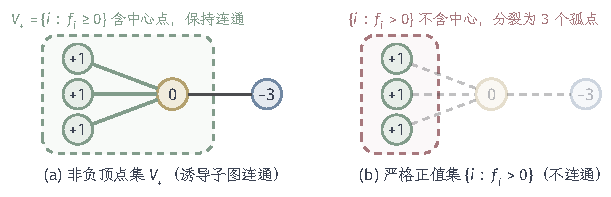
\includegraphics[width=103.396mm]{figures/03-graphs/05-matrices-and-spectra/tikz/fiedler-star-zero-center/figure.pdf}
  \caption{五顶点星图$K_{1,4}$上Fiedler向量$\bm f=(1,1,1,0,-3)^\top$的节域结构。(a) 非负集合$V_+=\{i:f_i\geq 0\}$包含取值为$0$的中心顶点，诱导子图保持连通；(b) 严格正值集合$\{i:f_i>0\}$不含中心顶点，分裂为三个孤立叶子。}
  \label{fig:graph-fiedler-star-zero}
\end{BookInlineFigure}

Fiedler向量$\bm v_2$通过一维连续坐标为所有顶点排出了反映瓶颈结构的自然顺序。在此基础上，接下来两节将进一步解决两个关键问题：第~\ref{sec:graph-cheeger}节引入归一化拉普拉斯与Cheeger不等式，严格证明沿谱方向扫描阈值必定能找到逼近全局最优导通率的稀疏割；第~\ref{sec:graph-ratiocut}至\ref{sec:graph-spectral-partition-comparison}节则给出RatioCut与NCut的完整谱划分算法。
